\chapter{General Notes}
\begin{itemize}
  \item Keep an eye on my blog\hyperlink{http://lextm.blogspot.com} and the
  project site\hyperlink{http://gforge.oss.org.cn/projects/codebeautifiers/}
  News will be published there.
  \item Please update the bundled Artistic Style and JEDI Code Format
  executables\footnote{for JCF, JCF2Settings.cfg in data$\backslash$config
  should be updated, too.}, by default, at C:$\backslash$Program
  Files$\backslash$Code Beautifier Collection 6$\backslash$bundled. Bundled
  versions are Artistic Style 1.21 and JEDI Code Format 2.24. There
  may be newer versions available at this moment.
  \label{links}
  \begin{itemize}

    \item Artistic Style, astyle.exe, is available on the web at \hyperlink{
    http://www.sourceforge.net/projects/astyle/ }
    \item JEDI Code Format command line version, jcf.exe, is available on the
    web at \hyperlink{http://jedicodeformat.sourceforge.net/ }

  \end{itemize}

  \item BDS should be closed before CBC installation and uninstallation
  processes. Install.exe will warn you.

  \item Without knowing its usage, don't delete any file in CBC installation
  folder, by default, at C:$\backslash$Program Files$\backslash$Code Beautifier
  Collection 6.

%   \item You may install extra Plus Packs to enjoy more features. Keep an eye on
%   CBC's homepage, and I will publish news there.
\end{itemize}

\chapter{IDE Versions Notes}
Code Beautifier Collection 6 only supports CodeGear RAD Studio 2007 IDE.
Previous IDE versions are not supported.
% \section{C\#Builder 1.0 Notes}
% \begin{itemize}
%   \item FileWizards feature of WiseEditor Plus is unavailable because of OTA
%   bugs.
%   \item AddMany features fails because of its implementation.
% \end{itemize}
% 
% \section{Delphi 2005 Notes}
% \begin{itemize}
%   \item The Code Beautifier Collection Delphi 2005 integration requires Delphi
%   2005 Update 1, 2, and 3. When loaded in the original release of Delphi 2005 it
%   causes AVs at startup.
% \end{itemize}

\chapter{CodeBeautifiers Plus Notes}
Project and Group menu items are disabled in this version. They may be
reimplemented in a later version.

% \subsection{AStyle Notes}
% The bundled version of AStyle is in Beta stage, which may not be stable
% sometimes. You may download and install the latest stable version yourself. I
% prefer this version because it fixes a few more bugs.

\section{JEDI Code Format Notes}
Sometimes when you format a broken Delphi source file, an error dialog shows.
In case that the dialog saying ''CBC is working'' is not closed automatically,
you can:
\begin{enumerate}
  \item Click on the white area of the dialog.
  \item Press Alt + F4.
\end{enumerate}
Then the dialog should be closed.

\section{XMLLex Notes}
All XML files parsed and formatted will be changed to UTF-8 encoding. If you
don't like this feature, do not use XMLLex to format your XML files at all.

I will try to fix this limitation in a later version.

\chapter{WiseEditor Plus Notes}
\begin{itemize}
  \item Because of an OTA bug, ComponentNamer fails sometimes. So it is disabled by
default. You can turn it on in Preferences Dialog.
  \item Because of CodeDOM limitations, Source Navigator only supports Delphi. 
  Also, constructors cannot be correctly located.
  \item DILMerge fails to resolve some projects. It is a bug of DILMerge so do
  not blame me.
\end{itemize}

\chapter{Shortcuts Notes}
\begin{itemize}
  \item It is Borland's convention that a shortcut is Delphi TShortcut-style
  value. So the value should be calculated carefully. This kind of calculation
  is valid for Delphi/C++Builder/Borland Developer Studio IDEs.
  \item It is normal that after customizing some shortcuts like Ctrl+D and
  Ctrl+E do not fired (usually they are already used by the IDE itself or some
  third party tools, like GExperts). You can change CBC shortcuts to remove
  these conflicts. Default value Ctrl+W for Beautify $|$ File menu item should
  be OK for most cases.
  \item You can only change a few shortcuts at run time. You cannot add a
  shortcut to a menu item without a shortcut before. That's the designer's
  intention.
\end{itemize}

\chapter{Icons Notes}
CBC uses icons including LeXtudio24.bmp, LeXtudio36.bmp, CBCOptionsMenu.bmp,
CodeBeautifiersFileMenu.bmp and so on.

LeXtudio files are originally made by lextm with MSPaint and GIMP.

Icons from the KidsXP icon set and Crystal icon set are used in CBC. And icons
for tools are taken from those tools directly using BeCyIconGrabber written by
Benjamin Bentmann (\underline{http://www.becyhome.de}). Thank you, Ben, for
creating this amazing utility.

Many images are taken from Customize.com. Because I cannot track and contact all
authors, if you are one of them and do not want your icons used in CBC please
contact me and I will stop using them.

% \chapter{Project Composition Notes}
%
% Figure~\ref{folder} provides details on how the project is composed.
%
% \begin{figure}[!hbp]
% \begin{center}
% 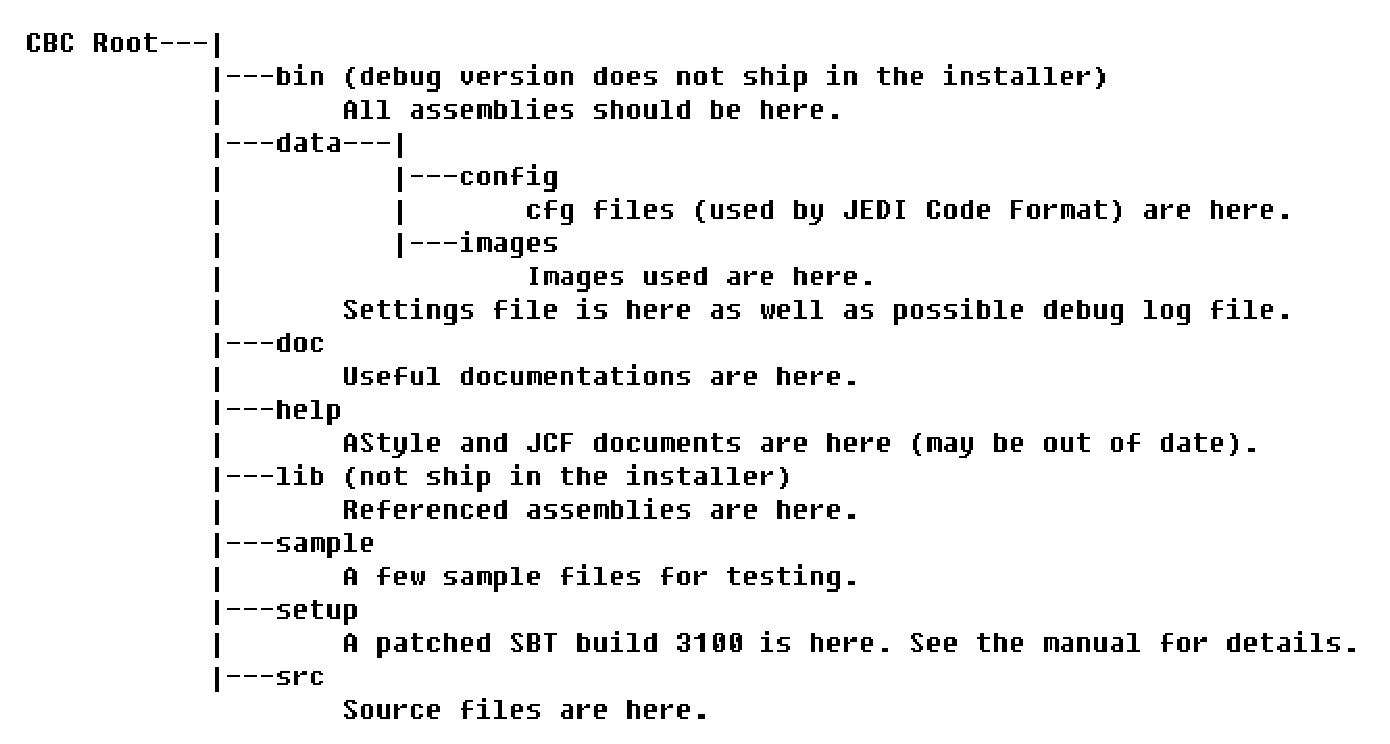
\includegraphics[width=1\textwidth]{images/Folders}
% \caption{Folder Tree of CBC} \label{folder}
% \end{center}
% \end{figure}

\chapter{Known Issues}
\begin{itemize}
  \item When newer versions of CBC try to load settings older versions
  left, there may be an error. As a result of this error, your settings may be
  corrupted. You have to manually set the preferences again. This issue will be
  addressed in a later version.

  \item Sometimes BDS freezes when launching if you switch to another window
  during the loading process. You have to kill bds.exe in the Windows Task
  Manager and restart it again.

  \item Most of other known bugs do not stop you from using CBC or damage your
  files.

  The bug tracker for this project is here

  \hyperlink{http://gforge.oss.org.cn/tracker/?atid=257}

  You are welcome to submit issues you meet there. Reported bugs will be fixed
  as soon as I could.

  \item Bugs of Artistic Style and JEDI Code Format should be posted to their
  bug tracker at SF.net. Refer to section \ref{links} for further information.
\end{itemize}
